\chapter{Analýza textov}\label{ch:textAnalysis}

Výskum sa zameriava na literárne diela dvoch autorov, Charlesa Dickensa a Oscara Wildea v dvoch jazykových variáciách: anglická a nemecká.
Cieľom je preskúmať vplyv interpunkcie na pozičnú slovnú sieť a jej mocninové rozdelenie.
Kapitola je rozdelená do štyroch hlavných častí: vývoj slovnej siete, distribúcia stupňov vrcholov, grafová analýza a jazyková analýza.

\section{Vývoj slovnej siete}\label{sec:vyvojSlovnejSiete}

Ako je možné vidieť na uvedených grafoch obr. č. \ref{fig:growthKoleda}, č. \ref{fig:growthTwist} a č. \ref{fig:growthDorian},
veľkosť exponentu mocninového rozdelenia $\gamma$ sa mení v závislosti od veľkosti siete. Pozorovanie vývoja slovných sietí vytvorených z literárnych diel v rôznych
jazykoch ukázalo, že rozdiel medzi slovnou sieťou bez interpunkcie a slovnou sieťou, ktorá obsahuje interpunkciu je najmä v počiatočnom
štádiu vývoja siete. 

V prípade Charlesa Dickensa sme analyzovali dve literárne diela, Vianočnú koledu a Olivera Twista. V oboch textoch, ako v anglickej, tak aj nemeckej verzii
boli najvýraznejšie zmeny exponentu $\gamma$ pozorované pri raste siete približne do veľkosti 1000 až 2000 vrcholov. Po prekročení tejto hranice sa hodnota exponentu postupne stabilizuje
a pohybuje sa v rozpätí $2$ až $2.2$.

Dielo Portrét Doriana Graya od Oscara Wildea bola analyzovaná rovnako v anglickej a nemeckej verzii. Aj v tomto prípade nastala najväčšia zmena hodnoty exponentu nastala pri raste siete do
veľkosti 1500 až 2000 vrcholov. Následne sa hodnota exponentu postupne stabilizovala a pohybovala sa v rovnakom rozpätí $2$ až $2.2$.

Na základe tejto analýzy boli identifikované dostatočne dlhé úseky textov, ktoré slúžili ako vstupné dáta pre nasledujúce analýzy.

\begin{figure}[htbp]
    \centering
    \begin{subfigure}[b]{0.9\textwidth}
        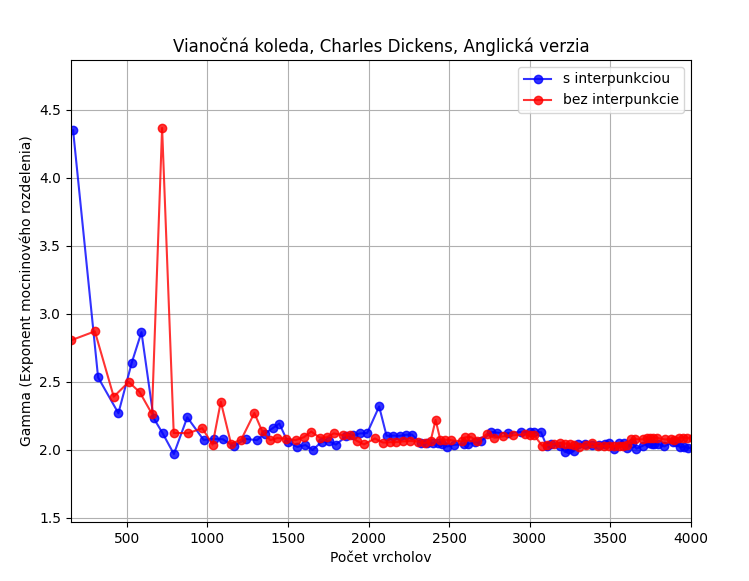
\includegraphics[width=\textwidth]{images/Growth/Screenshot_13.png}
    \end{subfigure}

    \vspace{0.3cm}

    \begin{subfigure}[b]{0.9\textwidth}
        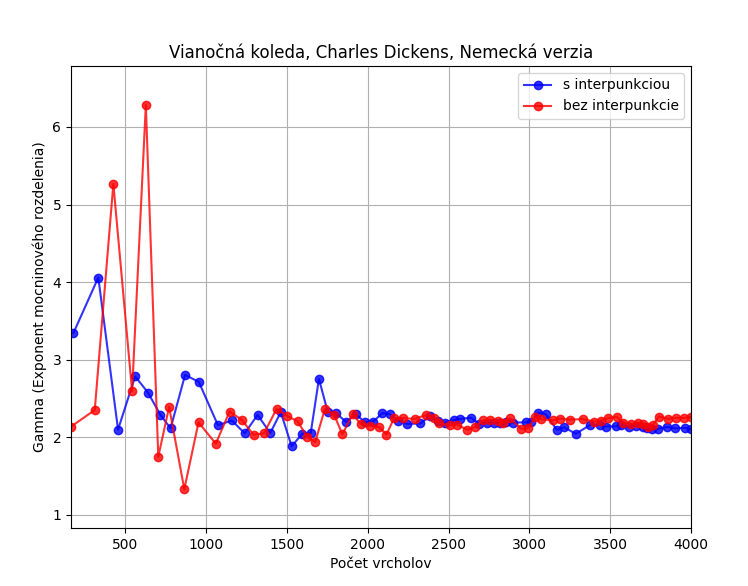
\includegraphics[width=\textwidth]{images/Growth/Screenshot_14.png}
    \end{subfigure}
    
    \vspace{0.3cm}
    \caption{Zmena veľkosti exponentu $\gamma$ v závisloti od veľkosti siete, text Vianočná koleda od Charlesa Dickensa.}\label{fig:growthKoleda}
\end{figure}

\begin{figure}[htbp]
    \centering
    \begin{subfigure}[b]{0.9\textwidth}
        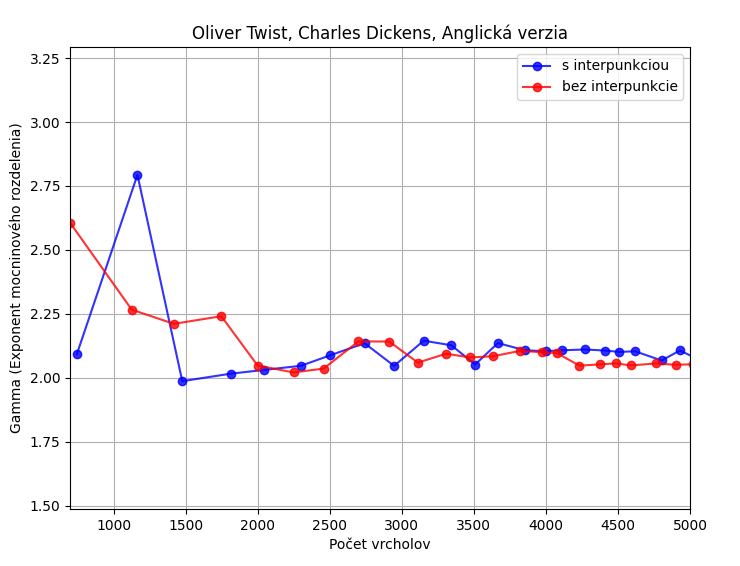
\includegraphics[width=\textwidth]{images/Growth/Screenshot_17.png}
    \end{subfigure}

    \vspace{0.3cm}

    \begin{subfigure}[b]{0.9\textwidth}
        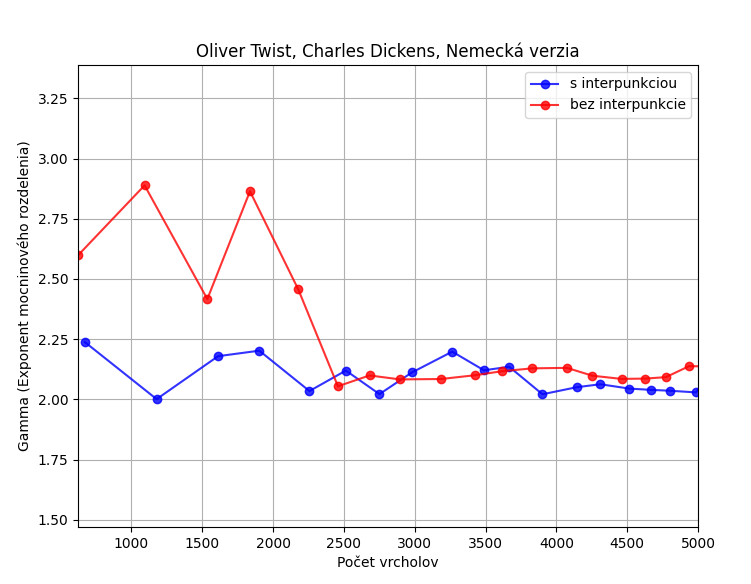
\includegraphics[width=\textwidth]{images/Growth/Screenshot_18.png}
    \end{subfigure}
    
    \vspace{0.3cm}
    \caption{Zmena veľkosti exponentu $\gamma$ v závisloti od veľkosti siete, text Oliver Twist od Charlesa Dickensa.}\label{fig:growthTwist}
\end{figure}

\begin{figure}[htbp]
    \centering
    \begin{subfigure}[b]{0.9\textwidth}
        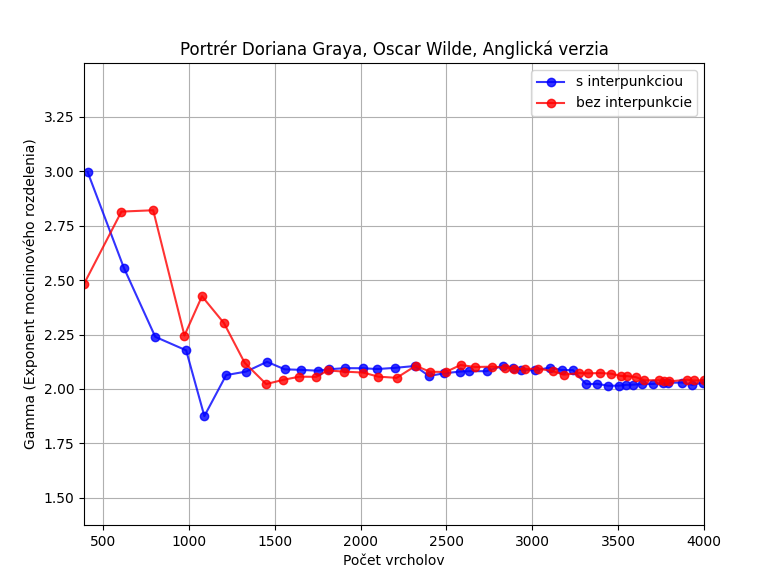
\includegraphics[width=\textwidth]{images/Growth/Screenshot_15.png}
    \end{subfigure}

    \vspace{0.3cm}

    \begin{subfigure}[b]{0.9\textwidth}
        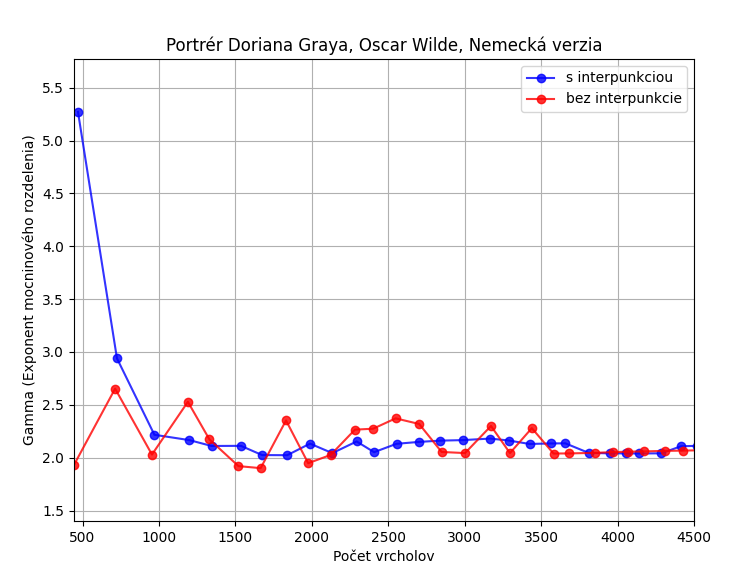
\includegraphics[width=\textwidth]{images/Growth/Screenshot_16.png}
    \end{subfigure}
    
    \vspace{0.3cm}
    \caption{Zmena veľkosti exponentu $\gamma$ v závisloti od veľkosti siete, text Portrét Doriana Graya od Oscara Wildea.}\label{fig:growthDorian}
\end{figure}

\clearpage

\section{Grafová analýza}\label{sec:grafovaAnalyza}

Grafová analýza textu pre slovnú sieť bez interpunkcie a so zohľadnením interpunkcie bola vykonaná na približne rovnako veľkých slovných sieťach.
Vo výsledkoch (tabuľka č. \ref{tab:anglickyBezInterpunkcie}, č. \ref{tab:anglickySInterpunkciou}, č. \ref{tab:nemeckyBezInterpunkcie} a č. \ref{tab:nemeckySInterpunkciou})
jednotlivých analýz môžeme pozorovať niekoľko zmien.

Ako si môžeme všimnúť, rozdiely sa opakovane prejavujú nezávisle od konkrétneho textu a jazyka. Rozdiely medzi slovnými sieťami bez interpunkcie a so zohľadnením interpunkcie
majú konzistentný charakter, pričom sa opakovane prejavuje rovnaký trend zmien v sledovaných parametroch.

Počet vrcholov a počet hrán sa v prípade oboch sietí mení len minimálne, zatiaľ čo maximálny stupeň v slovnej sieti s interpunkciou je výrazne vyšší, pretože
interpunkčné znamienka sú v porovnaní so slovami veľmi časté a vytvárajú tak väčší počet hrán. Napríklad čiarka alebo bodka sa môže spájať s mnohými slovami, čím vznikajú
uzly s vysokým stupňom. Vďaka tomu sa zvyšuje aj priemerný stupeň, ktorý je v prípade slovnej siete s interpunkciou vyšší, okrem textu Portrét Doriana Graya v angličtine, kde sa
priemerný stupeň znížil. 

Priemerný koeficient zhlukovania je v prípade slovnej siete s interpunkciou vyšší, čo naznačuje, že uzly sú v tejto sieti viac zoskupené do tzv. hubov. To vplýva aj na 
priemernú najkratšiu cestu, ktorá je v prípade slovnej siete s interpunkciou nižšia.

Ďalšie zaujímavé pozorovania sa týkajú korelácie medzi rôznymi typmi centrality:
\begin{itemize}
    \item Korelácia medzi stupňom a blízkosťou pohybujúca sa v intervale $0.34$ až $0.50$, ktorá udáva, ako blízko sú jednotlivé uzly.
          V prípade slovnej siete bez interpunkcie je vyššia.
    \item Korelácia medzi stupňom a medziľahlosťou je v oboch prípadoch veľmi vysoká v rozsahu $0.93$ až $0.96$ s minimálnou zmenou a naznačuje, že uzly s vysokým stupňom
          sú často aj uzlami, ktoré prepájajú rôzne časti siete.
    \item Korelácia medzi blízkosťou a medziľahlosťou je v prípade slovnej siete bez interpunkcie opäť vyššia, no vo všetkých prípadoch sa
          pohybuje v rozmedzí $0.23$ až $0.37$, čo naznačuje, že uzly majú slabú pozitívnu koreláciu medzi týmito dvoma typmi centrality. Tento výlsedok naznačuje, že uzly, ktoré sú blízko seba,
          nemusia zohrávať významnú úlohu pri tvorbe najkratších ciest v sieti.
\end{itemize}

Celkovo grafová analýza ukazuje, že interpunkcia má vplyv na štruktúru slovnej siete, čo sa prejave v rôznych parametroch siete, ako sú stupeň vrcholov, koeficient zhlukovania, priemerná najkratšia cesta
a korelácie medzi rôznymi typmi centrality.


\clearpage

\begin{table}[]
\centering
\scriptsize
\begin{tabular}{|c|c|c|c|}
\hline
\multicolumn{4}{|c|}{Grafová analýza, Anglický jazyk, bez interpunkcie} \\ \hline
\textbf{Text} &
  \begin{tabular}[c]{@{}c@{}}Vianočná koleda\\ $\sim$21000 slov\end{tabular} &
  \begin{tabular}[c]{@{}c@{}}Oliver Twist\\ $\sim$22000 slov\end{tabular} &
  \begin{tabular}[c]{@{}c@{}}Portrét Doriana Graya\\ $\sim$29000 slov\end{tabular} \\ \hline
Počet vrcholov & 3725 & 3842 & 3751 \\ \hline
Počet hrán & 14164 & 14762 & 17315 \\ \hline
\begin{tabular}[c]{@{}c@{}}Maximálny\\ stupeň\end{tabular} & 942 & 961 & 942 \\ \hline
\begin{tabular}[c]{@{}c@{}}Minimálny\\ stupeň\end{tabular} & 1 & 1 & 1 \\ \hline
\begin{tabular}[c]{@{}c@{}}Priemerný\\ stupeň\end{tabular} & 7.60483 & 7.68454 & 9.23220 \\ \hline
Hustota siete & 0.00204 & 0.00200 & 0.00246 \\ \hline
\begin{tabular}[c]{@{}c@{}}Korelácia centrality\\ (stupeň, blízkosť)\end{tabular} & 0.43094 & 0.42376 & 0.48416 \\ \hline
\begin{tabular}[c]{@{}c@{}}Korelácia centrality\\ (stupeň, medziľahlosť)\end{tabular} & 0.95007 & 0.95728 & 0.93399 \\ \hline
\begin{tabular}[c]{@{}c@{}}Korelácia centrality\\ (blízkosť, medziľahlosť)\end{tabular} & 0.29077 & 0.29174 & 0.31290 \\ \hline
\begin{tabular}[c]{@{}c@{}}Priemerný\\ koeficient\\ zhlukovania\end{tabular} & 0.35024 & 0.33708 & 0.34747 \\ \hline
\begin{tabular}[c]{@{}c@{}}Priemerná\\ najkratšia\\ cesta\end{tabular} & 2.91347 & 2.91189 & 2.86155 \\ \hline
Priemer & 7 & 8 & 7 \\ \hline
\end{tabular}
\caption{Grafová analýza, Anglický jazyk, bez interpunkcie}\label{tab:anglickyBezInterpunkcie}
\end{table}

\begin{table}[]
\centering
\scriptsize
\begin{tabular}{|c|c|c|c|}
\hline
\multicolumn{4}{|c|}{Grafová analýza, Anglický jazyk, s interpunkciou} \\ \hline
\textbf{Text} &
  \begin{tabular}[c]{@{}c@{}}Vianočná koleda\\ $\sim$21000 slov\end{tabular} &
  \begin{tabular}[c]{@{}c@{}}Oliver Twist\\ $\sim$22000 slov\end{tabular} &
  \begin{tabular}[c]{@{}c@{}}Portrét Doriana Graya\\ $\sim$29000 slov\end{tabular} \\ \hline
Počet vrcholov & 3737 & 3855 & 3761 \\ \hline
Počet hrán & 14389 & 14820 & 16934 \\ \hline
\begin{tabular}[c]{@{}c@{}}Maximálny\\ stupeň\end{tabular} & 1339 & 1215 & 1214 \\ \hline
\begin{tabular}[c]{@{}c@{}}Minimálny\\ stupeň\end{tabular} & 1 & 1 & 1 \\ \hline
\begin{tabular}[c]{@{}c@{}}Priemerný\\ stupeň\end{tabular} & 7.70083 & 7.68872 & 9.00505 \\ \hline
Hustota siete & 0.00206 & 0.00199 & 0.00239 \\ \hline
\begin{tabular}[c]{@{}c@{}}Korelácia centrality\\ (stupeň, blízkosť)\end{tabular} & 0.41137 & 0.40580 & 0.42678 \\ \hline
\begin{tabular}[c]{@{}c@{}}Korelácia centrality\\ (stupeň, medziľahlosť)\end{tabular} & 0.95424 & 0.96189 & 0.95068 \\ \hline
\begin{tabular}[c]{@{}c@{}}Korelácia centrality\\ (blízkosť, medziľahlosť)\end{tabular} & 0.27621 & 0.28199 & 0.27787 \\ \hline
\begin{tabular}[c]{@{}c@{}}Priemerný\\ koeficient\\ zhlukovania\end{tabular} & 0.44544 & 0.41362 & 0.44917 \\ \hline
\begin{tabular}[c]{@{}c@{}}Priemerná\\ najkratšia\\ cesta\end{tabular} & 2.77038 & 2.80452 & 2.73230 \\ \hline
Priemer & 6 & 6 & 7 \\ \hline
\end{tabular}
\caption{Grafová analýza, Anglický jazyk, s interpunkciou}\label{tab:anglickySInterpunkciou}
\end{table}

\begin{table}[]
\centering
\scriptsize
\begin{tabular}{|c|c|c|c|}
\hline
\multicolumn{4}{|c|}{Grafová analýza, Nemecký jazyk, bez interpunkcie} \\ \hline
\textbf{Text} &
  \begin{tabular}[c]{@{}c@{}}Vianočná koleda\\ $\sim$16000 slov\end{tabular} &
  \begin{tabular}[c]{@{}c@{}}Oliver Twist\\ $\sim$16000 slov\end{tabular} &
  \begin{tabular}[c]{@{}c@{}}Portrét Doriana Graya\\ $\sim$17000 slov\end{tabular} \\ \hline
Počet vrcholov & 3745 & 4133 & 3802 \\ \hline
Počet hrán & 12037 & 12287 & 12631 \\ \hline
\begin{tabular}[c]{@{}c@{}}Maximálny\\ stupeň\end{tabular} & 771 & 731 & 577 \\ \hline
\begin{tabular}[c]{@{}c@{}}Minimálny\\ stupeň\end{tabular} & 1 & 1 & 1 \\ \hline
\begin{tabular}[c]{@{}c@{}}Priemerný\\ stupeň\end{tabular} & 6.42830 & 5.94580 & 6.64440 \\ \hline
Hustota siete & 0.00172 & 0.00144 & 0.00175 \\ \hline
\begin{tabular}[c]{@{}c@{}}Korelácia centrality\\ (stupeň, blízkosť)\end{tabular} & 0.44845 & 0.43471 & 0.50290 \\ \hline
\begin{tabular}[c]{@{}c@{}}Korelácia centrality\\ (stupeň, medziľahlosť)\end{tabular} & 0.94554 & 0.95769 & 0.94727 \\ \hline
\begin{tabular}[c]{@{}c@{}}Korelácia centrality\\ (blízkosť, medziľahlosť)\end{tabular} & 0.31412 & 0.31849 & 0.36585 \\ \hline
\begin{tabular}[c]{@{}c@{}}Priemerný\\ koeficient\\ zhlukovania\end{tabular} & 0.21771 & 0.19410 & 0.22756 \\ \hline
\begin{tabular}[c]{@{}c@{}}Priemerná\\ najkratšia\\ cesta\end{tabular} & 3.20136 & 3.25713 & 3.19821 \\ \hline
Priemer & 9 & 9 & 7 \\ \hline
\end{tabular}
\caption{Grafová analýza, Nemecký jazyk, bez interpunkcie}\label{tab:nemeckyBezInterpunkcie}
\end{table}

\begin{table}[]
\centering
\scriptsize
\begin{tabular}{|c|c|c|c|}
\hline
\multicolumn{4}{|c|}{Grafová analýza, Nemecký jazyk, s interpunkciou} \\ \hline
\textbf{Text} &
  \begin{tabular}[c]{@{}c@{}}Vianočná koleda\\ $\sim$16000 slov\end{tabular} &
  \begin{tabular}[c]{@{}c@{}}Oliver Twist\\ $\sim$16000 slov\end{tabular} &
  \begin{tabular}[c]{@{}c@{}}Portrét Doriana Graya\\ $\sim$17000 slov\end{tabular} \\ \hline
Počet vrcholov & 3757 & 4145 & 3811 \\ \hline
Počet hrán & 12177 & 12546 & 12710 \\ \hline
\begin{tabular}[c]{@{}c@{}}Maximálny\\ stupeň\end{tabular} & 1271 & 1239 & 1060 \\ \hline
\begin{tabular}[c]{@{}c@{}}Minimálny\\ stupeň\end{tabular} & 1 & 1 & 1 \\ \hline
\begin{tabular}[c]{@{}c@{}}Priemerný\\ stupeň\end{tabular} & 6.48230 & 6.05356 & 6.67017 \\ \hline
Hustota siete & 0.00173 & 0.00146 & 0.00175 \\ \hline
\begin{tabular}[c]{@{}c@{}}Korelácia centrality\\ (stupeň, blízkosť)\end{tabular} & 0.34772 & 0.35362 & 0.39363 \\ \hline
\begin{tabular}[c]{@{}c@{}}Korelácia centrality\\ (stupeň, medziľahlosť)\end{tabular} & 0.95683 & 0.96393 & 0.95394 \\ \hline
\begin{tabular}[c]{@{}c@{}}Korelácia centrality\\ (blízkosť, medziľahlosť)\end{tabular} & 0.23112 & 0.24623 & 0.26092 \\ \hline
\begin{tabular}[c]{@{}c@{}}Priemerný\\ koeficient\\ zhlukovania\end{tabular} & 0.34032 & 0.30007 & 0.31879 \\ \hline
\begin{tabular}[c]{@{}c@{}}Priemerná\\ najkratšia\\ cesta\end{tabular} & 2.95941 & 3.03028 & 2.99317 \\ \hline
Priemer & 7 & 7 & 7 \\ \hline
\end{tabular}
\caption{Grafová analýza, Nemecký jazyk, s interpunkciou}\label{tab:nemeckySInterpunkciou}
\end{table}

\clearpage

\section{Distribúcia stupňov vrcholov}\label{sec:distribuciaStupnovvrcholov}

Distribúcia stupňov vrcholov bola analyzovaná pre úryvky textov, ktoré boli vybrané na základe vývoja slovnej siete \ref{sec:vyvojSlovnejSiete}. 
Skúmal sa vplyv zahrnutia interpunkcie do slovnej siete na mocninové rozdelenie stupňov vrcholov, zmenu exponentu $\gamma$ a podobnosť rozdelenia stupňov vrcholov
k teoretickému Dorogovtsev-Mendes modelu.

Výsledky sú zobrazené na obr. č. \ref{fig:lbdegdistKoleda}, č. \ref{fig:lbdegdistTwist} a č. \ref{fig:lbdegdistDorian} v podobe grafov 
zobrazujúcich rozdelenie stupňov vrcholov s využitím logaritmického zoskupovania v log-log mierke.
Na každom z týchto grafov je osobitne zobrazené rozdelenie pre sieť bez interpunkcie, s interpunkciou a teoretické rozdelenie Dorogovtsev-Mendes modelu.
Pre analýzu bolo potrebné odfiltrovať uzly s veľmi nízkym a vysokým stupňom, aby sa znížilo skreslenie výsledkov a vybrať najdlhšiu
klesajúcu časť charakteristiky pre výpočet hodnoty exponentu $\gamma$ mocninové rozdelenia.

Analýza ukázala, že slovné siete bez interpunkcie majú exponent $\gamma$ v rozmedzí $2.03$ až $2.16$ a slovné siete so zohľadnením interpunkcie
majú exponent $\gamma$ v intervale $2.02$ až $2.11$. Hodnoty $\gamma$ udávajú, že rozdelenie stupňov vrcholov v oboch prípadoch nasleduje 
mocninové rozdelenie, pričom hodnoty sa pohybujú v blízkosti $2$, čo je typické pre reálne siete. Taktiež dôvod prečo sa hodnoty exponentu $\gamma$
blížia k $2$ je ten, že v prípade slovných sietí vznikajú uzly s vysokým stupňom, zapríčinené častým výskytom spojok alebo predložiek, ktoré sa
často spájajú s inými slovami. Môžeme pozorovať, že v prípade slovnej siete s interpunkciou je hodnota exponentu $\gamma$ nižšia vo všetkých prípadoch,
pretože interpunkčné znamienka majú tendenciu vytvárať uzly s vysokým stupňom.

Porovnanie s teoretickým Dorogovtsev-Mendes modelom sa uskutočnilo na základe hodnoty strednej kvadratickej chyby normalizovanej distribúcie stupňov vrcholov,
ktorá sa pohybuje v rozmedzí $0.00022$ až $0.00028$ pre sieť bez interpunkcie a $0.00015$ až $0.00021$ pre sieť s interpunkciou.

Zistenia potvrdzujú, že rozdelenie stupňov vrcholov v slovných sieťach s interpunkciou aj bez nej vykazuje charakteristiky bezškálových sietí a výraznú
podobnosť s teoretickým Dorogovtsev-Mendes modelom.



\begin{figure}[htbp]
    \centering
    \begin{subfigure}[b]{0.9\textwidth}
        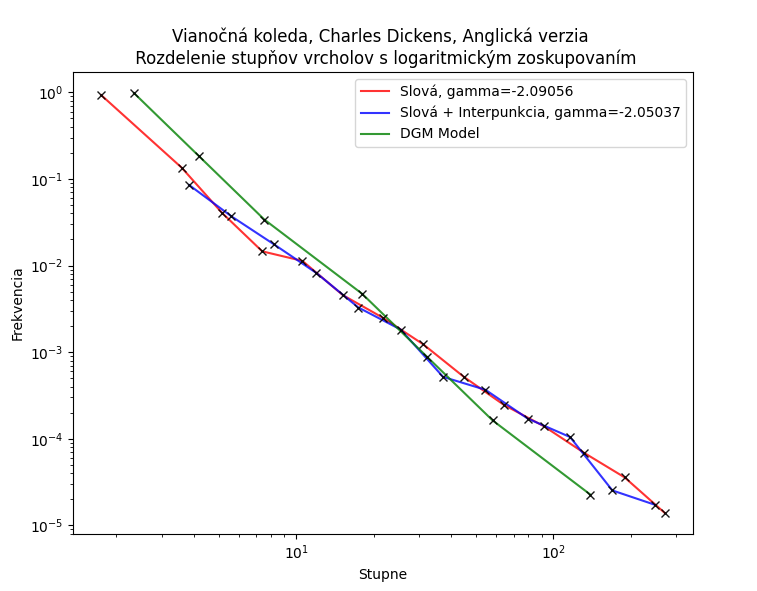
\includegraphics[width=\textwidth]{images/lbdegdist/Screenshot_1.png}
    \end{subfigure}

    \vspace{0.3cm}

    \begin{subfigure}[b]{0.9\textwidth}
        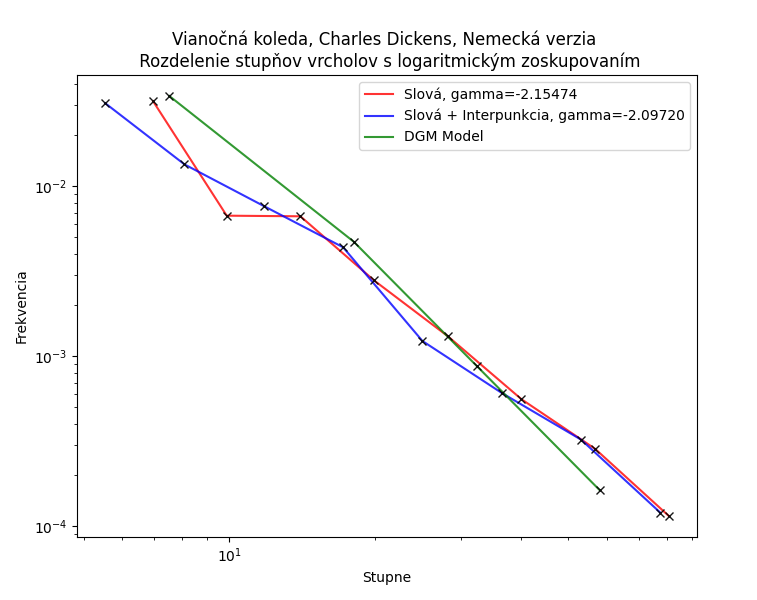
\includegraphics[width=\textwidth]{images/lbdegdist/Screenshot_2.png}
    \end{subfigure}
    
    \vspace{0.3cm}
    \caption{Distribúcia stupňov vrcholov s využitím logaritmického zoskupovania, text Vianočná koleda od Charlesa Dickensa.}\label{fig:lbdegdistKoleda}
\end{figure}

\begin{figure}[htbp]
    \centering
    \begin{subfigure}[b]{0.9\textwidth}
        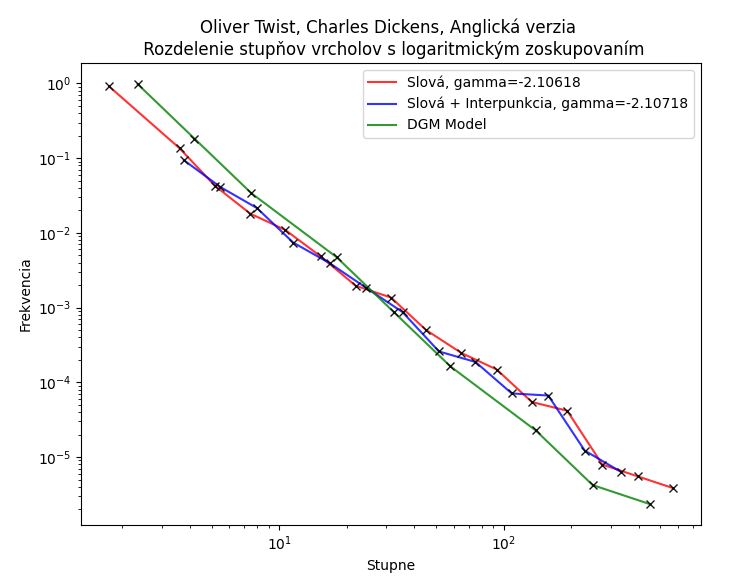
\includegraphics[width=\textwidth]{images/lbdegdist/Screenshot_5.png}
    \end{subfigure}

    \vspace{0.3cm}

    \begin{subfigure}[b]{0.9\textwidth}
        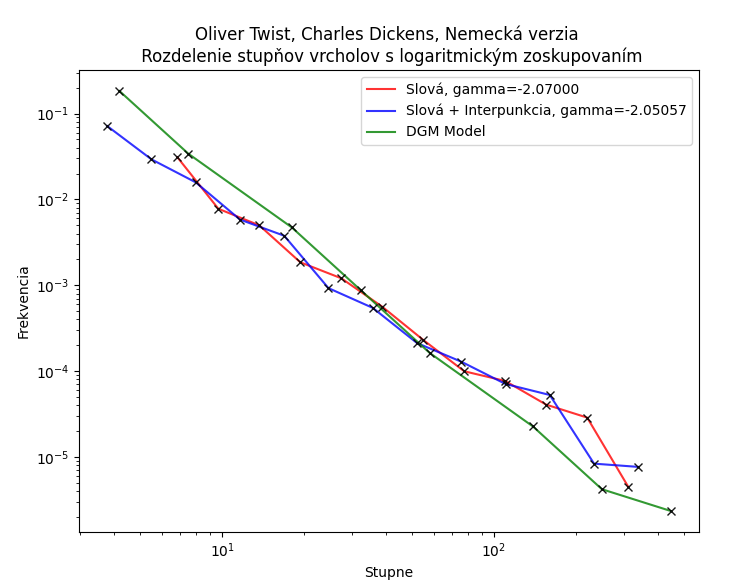
\includegraphics[width=\textwidth]{images/lbdegdist/Screenshot_6.png}
    \end{subfigure}
    
    \vspace{0.3cm}
    \caption{Distribúcia stupňov vrcholov s využitím logaritmického zoskupovania, text Oliver Twist od Charlesa Dickensa.}\label{fig:lbdegdistTwist}
\end{figure}

\begin{figure}[htbp]
    \centering
    \begin{subfigure}[b]{0.9\textwidth}
        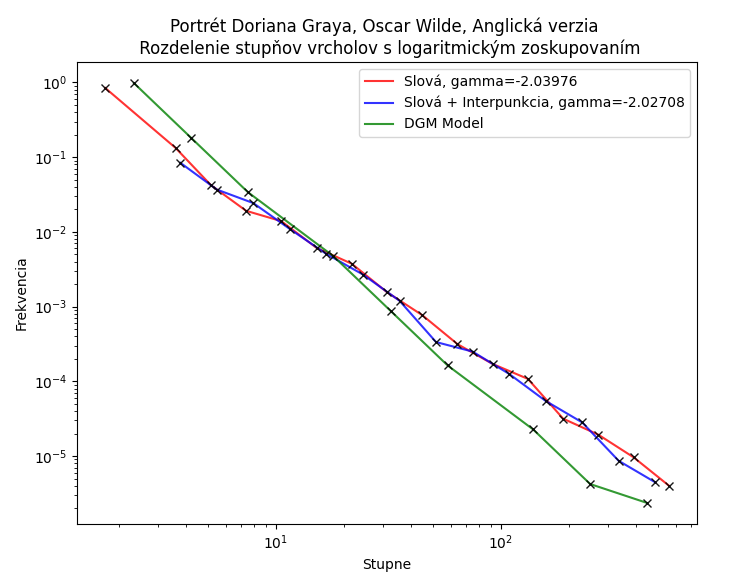
\includegraphics[width=\textwidth]{images/lbdegdist/Screenshot_3.png}
    \end{subfigure}

    \vspace{0.3cm}

    \begin{subfigure}[b]{0.9\textwidth}
        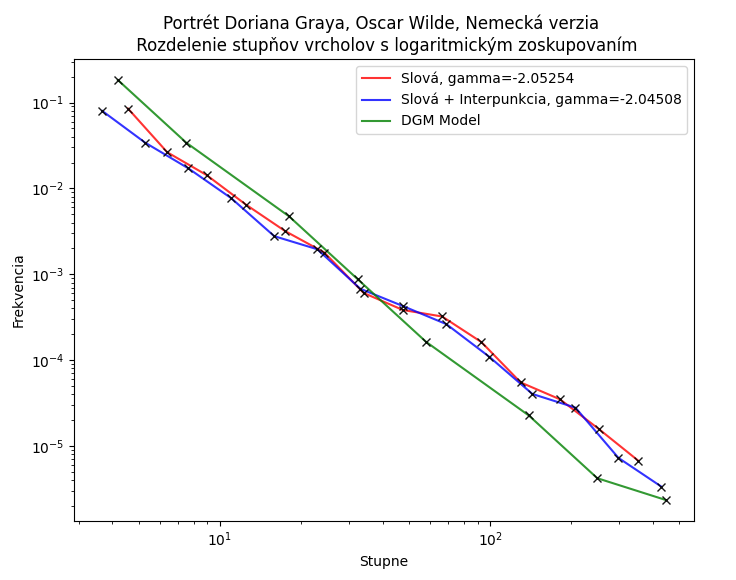
\includegraphics[width=\textwidth]{images/lbdegdist/Screenshot_4.png}
    \end{subfigure}
    
    \vspace{0.3cm}
    \caption{Distribúcia stupňov vrcholov s využitím logaritmického zoskupovania, text Portrét Doriana Graya od Oscara Wildea.}\label{fig:lbdegdistDorian}
\end{figure}

\clearpage

\section{Jazyková analýza}\label{sec:jazykovaAnalyza}

Jazyková analýza jednotlivých diel bola vykonaná na slovných sieťach so zohľadnením interpunkcie.
V tabuľkách č. \ref{tab:anglickyJazykovaAnalyza} a č. \ref{tab:nemeckyJazykovaAnalyza} sú uvedené výsledky jazykovej analýzy pre anglický a nemecký jazyk.
Možno pozorovať viaceré rozdiely, ktoré sú spôsobené štruktúrou jazykov a štýlom prekladu.

Počet interpunkčných znakov sa v jednotlivých dielach výrazne líši, aj napriek tomu, že analyzované slovné siete sú približne rovnakej veľkosti.
Tento rozdiel je zapríčinený tým, že na vytvorenie slovnej siete určitej veľkosti je potrebné odlišné množstvo textu. Množstvo textu je závislé od
štruktúry samostatného jazyka a štýlom písania autora či prekladateľa. Ak si vypočítame pomer medzi veľkosťou vzorky textu a počtom interpunkčných znakov,
zistíme, že v prípade anglického jazyka sa tento pomer pohybuje v intervale $4.8$ až $5.1$ a v prípade nemeckého jazyka $5.2$ až $5.4$.
Tento pomer ukazuje, že vo všetkých dielach v oboch jazykoch je počet interpunkčných znakov v priemere približne päťkrát menší, ako počet slov.

Priemerná dĺžka slova je vyššia pre všetky analýzy v nemeckom jazyku (okolo $7.5$ až $7.9$ znakov), čo je typické pre nemecký jazyk, v ktorom sa
často vyskytujú dlhé zložené slová. V anglickom jazyku sa priemerná dĺžka slova pohybuje v rozmedzí $6.4$ až $6.7$ znakov. Rovnaký 
trend je pozorovaný aj v prípade maximálnej dĺžky slova, ktorá sa v nemeckom jazyku pohybuje v rozmedzí $23$ až $26$ znakov, zatiaľ čo v anglickom jazyku
sa maximálna dĺžka slova pohybuje v intervale $15$ až $16$ znakov.

Štatistiky týkajúce sa dĺžky viet vykazujú podobné hodnoty, jediný výrazný rozdiel je v maximálnej dĺžke vety textu Oliver Twist, kde je v anglickom jazyku
viac ako dvojnásobná v porovnaní s nemeckým prekladom. Tento rozdiel môže byť spôsobený viacerými faktormi, ako sú štruktúra jazyka či preklad textu.	

Taktiež sa skúmal výskyt dvojíc a trojíc slov v textoch, ktoré tvoria časté slovné spojenia. Táto analýza silno závisí od štýlu písania autora, štruktúry a veľkosti textu, ako
vidno v anglickej verzii Portrétu Doriana Graya, kde sa vyskytuje najviac dvojíc a trojíc slov. Dôvodom môže byť aj veľkosť textu, ktorý je v porovnaní s ostatnými anglickými textami
o takmer $30\%$ väčší. Veľkú úlohu zohráva aj gramatická štruktúra jazyka, ktorá ovplyvňuje výskyt dvojíc a trojíc slov, pretože pravidlá písania napríklad čiarky môže vytvárať
dvojice, trojice uzlov s vysokou frekvenciou.

Tieto zistenia naznačujú, že jazyková analýza môže poskytnúť cenné informácie o štruktúre a charakteristikách textu, ako aj o štýle písania autora.

\clearpage

\begin{table}[]
\centering
\scriptsize
\begin{tabular}{|c|c|c|c|}
\hline
\multicolumn{4}{|c|}{Jazyková analýza, Anglický jazyk} \\ \hline
\textbf{Veľkosť textu (slová)} &
  \begin{tabular}[c]{@{}c@{}}Vianočná koleda\\ $\sim$21000 slov\end{tabular} &
  \begin{tabular}[c]{@{}c@{}}Oliver Twist\\ $\sim$22000 slov\end{tabular} &
  \begin{tabular}[c]{@{}c@{}}Portrét Doriana Graya\\ $\sim$29000 slov\end{tabular} \\ \hline
Počet interpunkčných znamienok & 4377 & 4350 & 5782 \\ \hline
Najväčší výskyt interpunkčného znamienka & 2055 & 2123 & 2302 \\ \hline
Najmenší výskyt interpunkčného znamienka & 47 & 38 & 16 \\ \hline
Počet unikátnych slov & 3737 & 3855 & 3761 \\ \hline
Maximálna dĺžka slova & 15 & 15 & 16 \\ \hline
Minimálna dĺžka slova & 1 & 1 & 1 \\ \hline
Priemerná dĺžka slova & 6.45063 & 6.73281 & 6.56076 \\ \hline
Počet viet & 1329 & 1425 & 2612 \\ \hline
Maximálna dĺžka vety & 136 & 209 & 124 \\ \hline
Minimálna dĺžka vety & 1 & 1 & 1 \\ \hline
Priemerná dĺžka vety & 15.99473 & 15.80561 & 11.38055 \\ \hline
Počet dvojíc slov & 15057 & 15363 & 17700 \\ \hline
Maximálna frekvencia dvojice & 400 & 309 & 618 \\ \hline
Minimálna frekvencia dvojice & 1 & 1 & 1 \\ \hline
Priemerná frekvencia dvojice & 1.78409 & 1.83616 & 2.09960 \\ \hline
Počet trojíc slov & 22956 & 23647 & 29482 \\ \hline
Maximálna frekvencia trojice & 73 & 119 & 256 \\ \hline
Minimálna frekvencia trojice & 1 & 1 & 1 \\ \hline
Priemerná frekvencia trojice & 1.17015 & 1.19288 & 1.26050 \\ \hline
\end{tabular}
\caption{Jazyková analýza, Anglický jazyk}\label{tab:anglickyJazykovaAnalyza}
\end{table}


\begin{table}[]
\centering
\scriptsize
\begin{tabular}{|c|c|c|c|}
\hline
\multicolumn{4}{|c|}{Jazyková analýza, Nemecký jazyk} \\ \hline
\textbf{Veľkosť textu (slová)} &
  \begin{tabular}[c]{@{}c@{}}Vianočná koleda\\ $\sim$16000 slov\end{tabular} &
  \begin{tabular}[c]{@{}c@{}}Oliver Twist\\ $\sim$16000 slov\end{tabular} &
  \begin{tabular}[c]{@{}c@{}}Portrét Doriana Graya\\ $\sim$17000 slov\end{tabular} \\ \hline
Počet interpunkčných znamienok & 2983 & 2973 & 3224 \\ \hline
Najväčší výskyt Interpunkčného znamienka & 1703 & 1606 & 1580 \\ \hline
Najmenší výskyt Interpunkčného znamienka & 8 & 24 & 25 \\ \hline
Počet unikátnych slov & 3757 & 4145 & 3811 \\ \hline
Maximálna dĺžka slova & 23 & 26 & 24 \\ \hline
Minimálna dĺžka slova & 1 & 1 & 1 \\ \hline
Priemerná dĺžka slova & 7.58957 & 7.91870 & 7.89766 \\ \hline
Počet viet & 1035 & 1041 & 1417 \\ \hline
Maximálna dĺžka vety & 126 & 90 & 114 \\ \hline
Minimálna dĺžka vety & 1 & 1 & 1 \\ \hline
Priemerná dĺžka vety & 15.49758 & 15.25456 & 11.93719 \\ \hline
Počet dvojíc slov & 12703 & 13039 & 13229 \\ \hline
Maximálna frekvencia dvojice & 188 & 163 & 204 \\ \hline
Minimálna frekvencia dvojice & 1 & 1 & 1 \\ \hline
Priemerná frekvencia dvojice & 1.56050 & 1.50732 & 1.58644 \\ \hline
Počet trojíc slov & 17742 & 17706 & 18599 \\ \hline
Maximálna frekvencia trojice & 87 & 53 & 155 \\ \hline
Minimálna frekvencia trojice & 1 & 1 & 1 \\ \hline
Priemerná frekvencia trojice & 1.11724 & 1.10996 & 1.12834 \\ \hline
\end{tabular}
\caption{Jazyková analýza, Nemecký jazyk}\label{tab:nemeckyJazykovaAnalyza}
\end{table}